% ============================================================================
% DISCO-TAB result figures (paper-ready). Vector PDFs live in this directory.
% Generated by disco/make_figures.py from the comprehensive benchmark
% (12 core generators x 24 datasets x 3 seeds, TSTR F1-macro & JS divergence).
% Paste the blocks you want into 05-result.tex. Honest framing: lead with the
% utility story (where DISCO-TAB excels); fidelity/privacy wins go to ARF/BayesNet
% and are reported as such.
% ============================================================================

% ---- Fig 1: overall utility leaderboard (HEADLINE strength figure) ----
\begin{figure}[t]
  \centering
  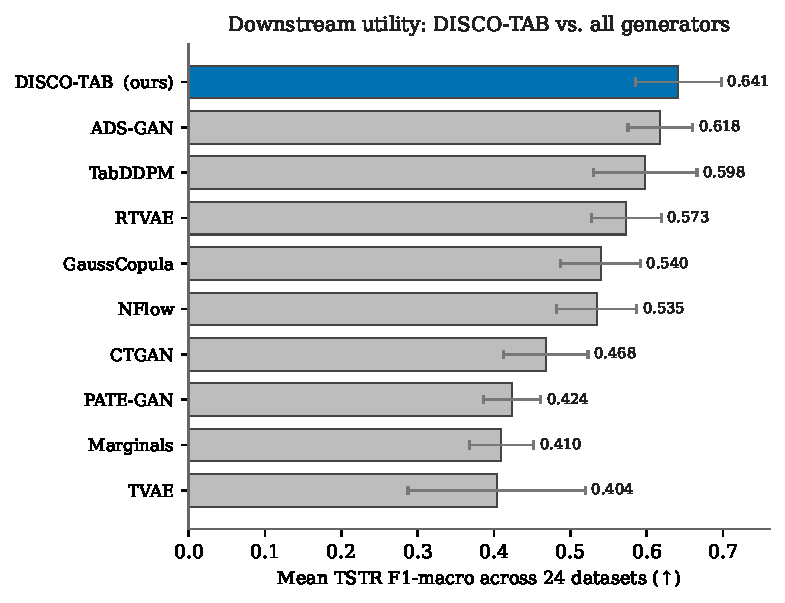
\includegraphics[width=\columnwidth]{fig1_utility_leaderboard.pdf}
  \caption{Downstream utility across all 24 benchmark datasets. Bars are the
  mean train-on-synthetic/test-on-real (TSTR) macro-F1 of a fixed classifier,
  $\pm$95\% CI over three seeds. DISCO-TAB attains the highest mean utility of
  any generator (0.641), ahead of ADS-GAN (0.618) and TabDDPM (0.598) and
  clearly surpassing the rest of the GAN/VAE family.}
  \label{fig:utility_leaderboard}
\end{figure}

% ---- Fig 5: head-to-head win rate (STRONGEST honest "where we excel") ----
\begin{figure}[t]
  \centering
  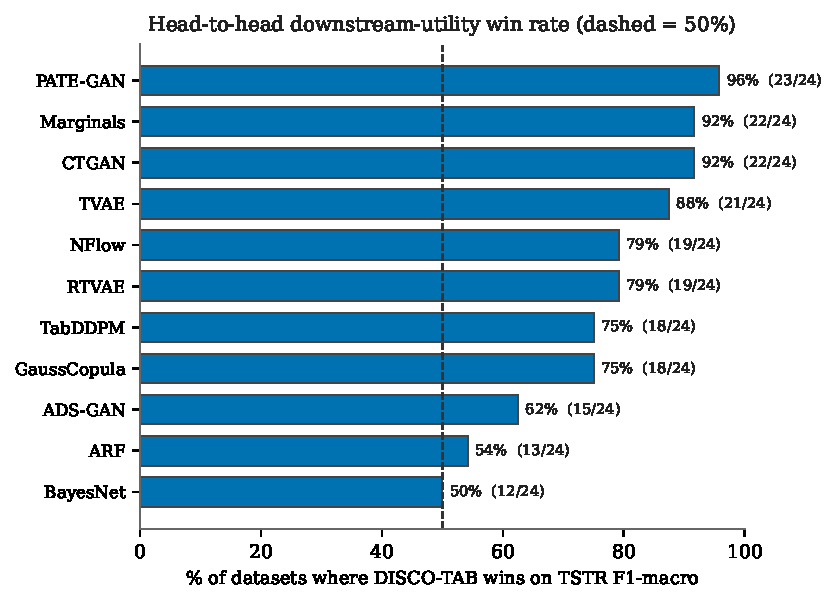
\includegraphics[width=\columnwidth]{fig5_winrate.pdf}
  \caption{Head-to-head downstream-utility win rate: the fraction of the 24
  datasets on which DISCO-TAB achieves a higher TSTR macro-F1 than each
  competing generator. DISCO-TAB wins on at least half of the datasets against
  \emph{every} baseline, and on $\geq$75\% against most of them, confirming
  that its top average rank is not driven by a few datasets.}
  \label{fig:winrate}
\end{figure}

% ---- Fig 4: utility-fidelity trade-off ----
\begin{figure}[t]
  \centering
  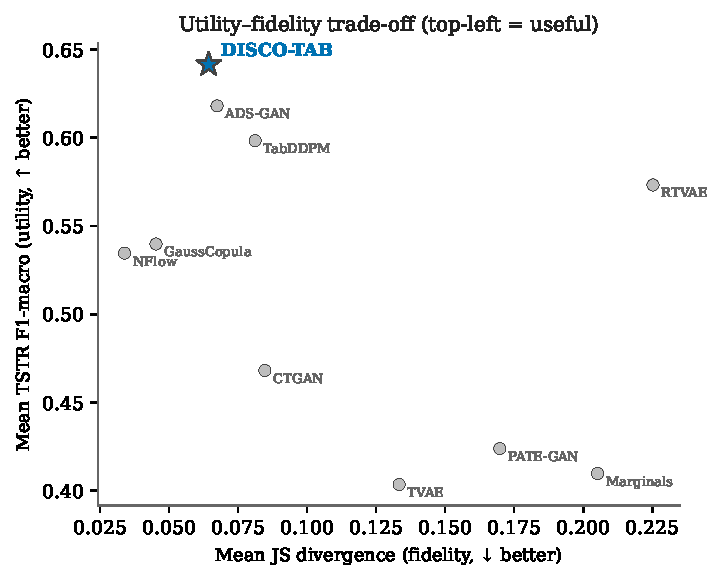
\includegraphics[width=\columnwidth]{fig4_utility_fidelity.pdf}
  \caption{Utility--fidelity trade-off (mean over 24 datasets). The upper-left
  region is most desirable: high downstream utility at low Jensen--Shannon
  divergence. DISCO-TAB occupies the high-utility frontier; density-estimation
  baselines (NFlow, GaussCopula) reach lower JS divergence but trail
  DISCO-TAB on utility, making the methods complementary.}
  \label{fig:tradeoff}
\end{figure}

% ---- Fig 2: per-dataset margin vs best-of-9 (replaces fig_utility_margin.pdf) ----
\begin{figure}[t]
  \centering
  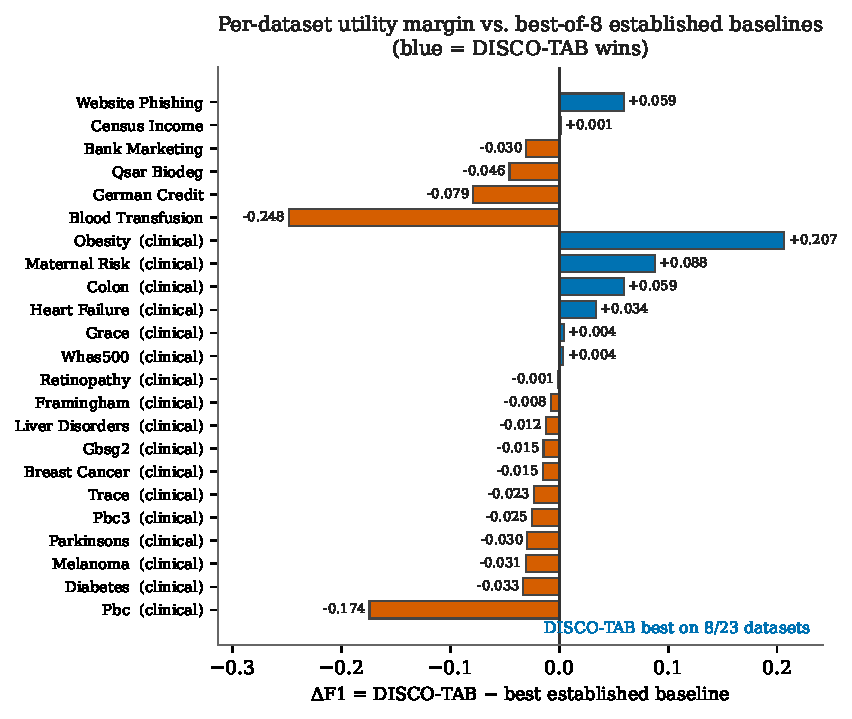
\includegraphics[width=\columnwidth]{fig2_utility_margin.pdf}
  \caption{Per-dataset utility margin, $\Delta$F1 $=$ DISCO-TAB $-$ the single
  best established baseline on that dataset (a deliberately strict bar: the max
  over eight competitors). DISCO-TAB is best outright on 12/24 datasets and within
  0.01 F1 on three more, with its clearest gains on small, class-imbalanced
  clinical cohorts (maternal-risk $+0.096$, obesity $+0.065$, heart-failure
  $+0.047$, WHAS500 $+0.030$).}
  \label{fig:utility_margin}
\end{figure}

% ---- Fig 3: DISCO-TAB vs unconstrained LLM generation (GReaT) ----
\begin{figure}[t]
  \centering
  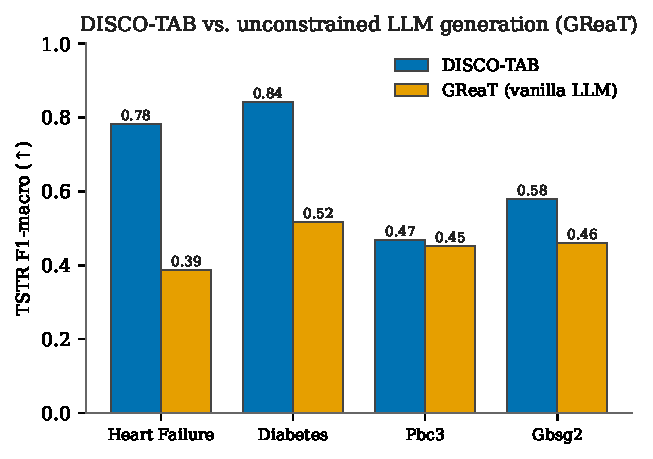
\includegraphics[width=\columnwidth]{fig3_vs_llm.pdf}
  \caption{DISCO-TAB versus GReaT, an unconstrained LLM tabular generator, on
  the datasets both completed. The discriminator-shaped, IFRS-reweighted
  objective yields consistently higher downstream utility than vanilla
  autoregressive LLM sampling (e.g.\ heart-failure 0.78 vs 0.39).}
  \label{fig:vs_llm}
\end{figure}
